\section{Additional experimental details}
\label{supp:experiments}

Table~\ref{tab:corrlevel} reports the per-statistic rejection rates of
the hollow test on Fisher-$z$ sample-correlation networks built from
$T\times n$ panels of i.i.d.\ $N(0,1)$ entries ($n=120$, $R=100$
replicates, $B=99$), complementing the combined rates quoted in the main
text. The size of every statistic is within Monte Carlo error of the
nominal $0.05$ at both panel lengths.

\begin{table}[h]
\centering\small
\caption{Empirical size at nominal $0.05$ of the hollow test on
finite-$T$ sample-correlation networks (isotropic Gaussian panels,
$n=120$, $R=100$, $B=99$).}
\label{tab:corrlevel}
\begin{tabular}{lcccccc}
\toprule
 & IPR & eigenvector KS & clustering & strength CV & kurtosis & combined\\
\midrule
$T=120$ & 0.01 & 0.06 & 0.06 & 0.00 & 0.00 & 0.060\\
$T=360$ & 0.03 & 0.06 & 0.03 & 0.00 & 0.01 & 0.040\\
\bottomrule
\end{tabular}
\end{table}

Two conventions used in Section~\ref{sec:exp-heavy} of the main text
deserve elaboration. The synthetic ensembles are tested as full matrices
because their models specify diagonals, and only the genuinely hollow
air-traffic data pass through the hollow pipeline. The distinction
matters for extremely heavy spectra: zeroing the diagonal of a Haar
replicate subtracts a diagonal matrix whose entries fluctuate on the
scale of the root mean square of the spectrum, and when a few eigenvalues
dominate that scale, the subtraction itself localizes the replicate
eigenvectors attached to small eigenvalues. The pipeline is exact for full matrices and approximate for hollow
data in either convention (Remark~3 of the main text), and the
upper-tail reading of the IPR statistic is most interpretable when the
convention matches the data, which is how the experiments are run.

\begin{figure}[h]
\centering
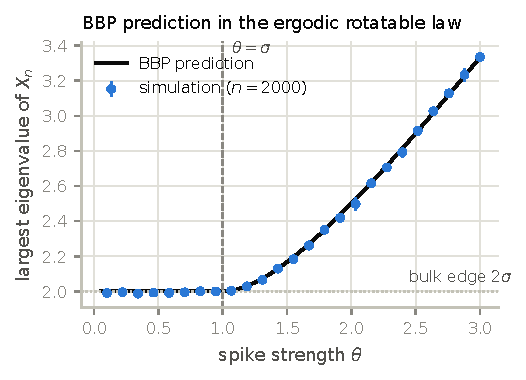
\includegraphics[width=0.55\textwidth]{figures/figS2_bbp_check.pdf}
\caption{Largest eigenvalue of the ergodic law versus spike strength
($n=2000$; mean $\pm$ s.d.\ over 6 replicates) against the prediction
of Proposition~S2; the transition is at $\theta=\sigma$.}
\label{fig:bbpcheck}
\end{figure}

\begin{figure}[h]
\centering
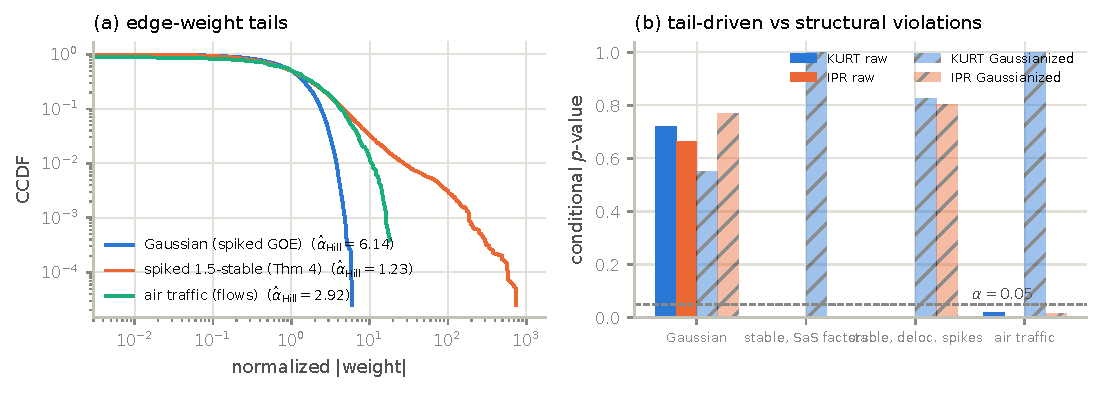
\includegraphics[width=\textwidth]{figures/fig5_heavy.pdf}
\caption{Heavy tails. (a) CCDFs of normalized edge weights with Hill
indices: spiked GOE, the spiked $1.5$-stable law of
Theorem~\ref{thm:stable}, and air traffic. (b) Conditional $p$-values
of kurtosis and IPR, raw and after Gaussianization, for the Gaussian
control, the $\SaS$-factor model, the delocalized-spike control, and
air traffic (first tie seed shown; ranges in Table~\ref{tab:real} and
text).}
\label{fig:heavy}
\end{figure}

\begin{table}[h]
\centering\small
\caption{Rejection rates at nominal $0.05$ of three null models under
the same rotatable truth (spiked GOE, $0$--$3$ random spikes, $n=120$,
$R=100$, $B=99$, hollow pipeline). The Haar-conditional row is the
level study of Figure~2(a) ($R=250$).}
\label{tab:baselines}
\begin{tabular}{lcccccc}
\toprule
Null model & IPR & eigenvector KS & clustering & strength CV & kurtosis & combined\\
\midrule
Haar-conditional (this paper) & \multicolumn{5}{c}{uniform $p$-values (Fig.~2a)} & 0.068\\
Weight permutation & 0.07 & 0.05 & 0.57 & 0.42 & 0.00 & 0.51\\
Fitted-spike parametric bootstrap & 0.02 & 0.07 & 0.10 & 0.03 & 0.06 & 0.03\\
\bottomrule
\end{tabular}
\end{table}
